\chapter{Bonus: Tutorial}
\section{How to classify your own images of digits}
This tutorial will guide you on how to use the classifier provided in exercise 3 to classify you own images like figure \ref{fig:w5_imgclass}:

\begin{figure}[ht]
\center
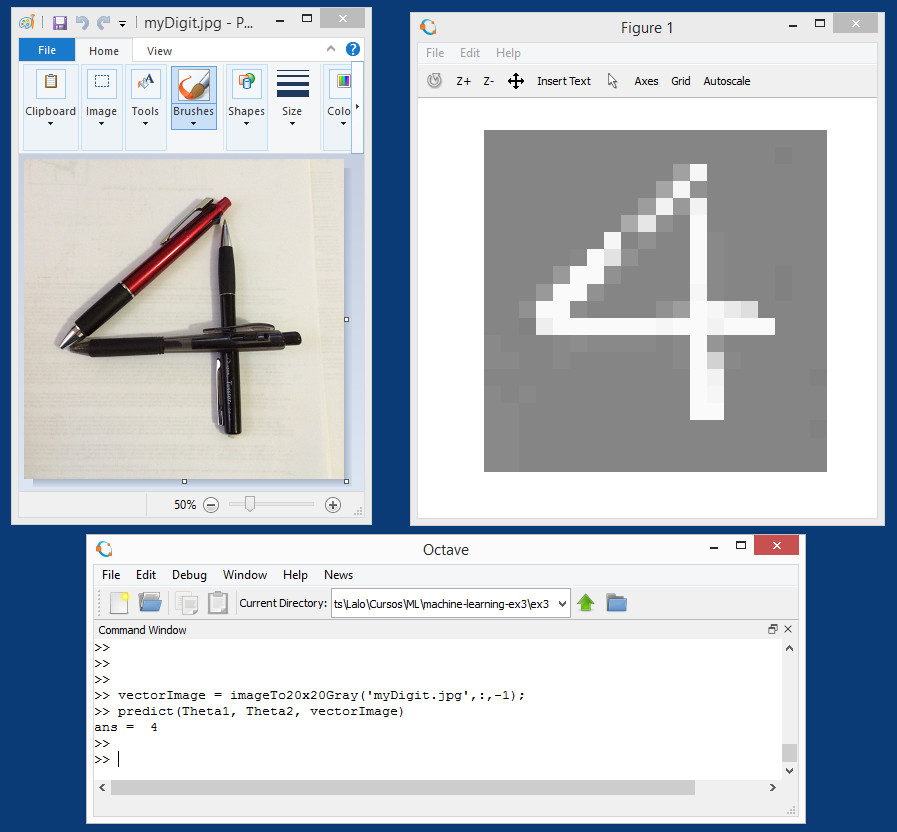
\includegraphics[scale=0.3]{W5_imgclass}
\caption{Image classifier}
\label{fig:w5_imgclass}
\end{figure}
It will also explain how the images are converted thru several formats to be processed and displayed.
\section{Introduction}
The classifier provided expects 20 x 20 pixels black and white images converted in a row vector of 400 real numbers like this:
\begin{verbatim}
[ 0.14532, 0.12876, ...]
\end{verbatim}
Each pixel is represented by a real number between -1.0 to 1.0, meaning -1.0 equal black and 1.0 equal white (any number in between is a shade of gray, and number 0.0 is exactly the middle gray).
\section{.jpg and color RGB images}
The most common image format that can be read by Octave is .jpg using function that outputs a three-dimensional matrix of integer numbers from 0 to 255, representing the height x width x 3 integers as indexes of a color map for each pixel (explaining color maps is beyond scope).

\begin{verbatim}
Image3DmatrixRGB = imread("myOwnPhoto.jpg");
\end{verbatim}

\section{Convert to Black \& White}
A common way to convert color images to black \& white, is to convert them to a YIQ standard and keep only the Y component that represents the luma information (black \& white). I and Q represent the chrominance information (color).Octave has a function \verb|rgb2ntsc()| that outputs a similar three-dimensional matrix but of real numbers from -1.0 to 1.0, representing the height x width x 3 (Y luma, I in-phase, Q quadrature) intensity for each pixel.
\begin{verbatim}
Image3DmatrixYIQ = rgb2ntsc(MyImageRGB);
\end{verbatim}
To obtain the Black \& White component just discard the I and Q matrices. This leaves a two-dimensional matrix of real numbers from -1.0 to 1.0 representing the height x width pixels black \& white values.
\begin{verbatim}
Image2DmatrixBW = Image3DmatrixYIQ(:,:,1);
\end{verbatim}
\section{Cropping to square image}
It is useful to crop the original image to be as square as possible. The way to crop a matrix is by selecting an area inside the original B\&W image and copy it to a new matrix. This is done by selecting the rows and columns that define the area. In other words, it is copying a rectangular subset of the matrix like this:
\begin{verbatim}
croppedImage = Image2DmatrixBW(origen1:size1, origin2:size2);
\end{verbatim}
Cropping does not have to be all the way to a square. \textbf{It could be cropping just a percentage of the way to a square} so you can leave more of the image intact. The next step of scaling will take care of streaching the image to fit a square.
\section{Scaling to 20 x 20 pixels}
The classifier provided was trained with 20 x 20 pixels images so we need to scale our photos to meet. It may cause distortion depending on the height and width ratio of the cropped original photo. There are many ways to scale a photo but we are going to use the simplest one. We lay a scaled grid of 20 x 20 over the original photo and take a sample pixel on the center of each grid. To lay a scaled grid, we compute two vectors of 20 indexes each evenly spaced on the original size of the image. One for the height and one for the width of the image. For example, in an image of 320 x 200 pixels will produce to vectors like
\begin{verbatim}
[9    25    41    57    73 ... 313] % 20 indexes

[6    16    26    36    46 ... 196] % 20 indexes
\end{verbatim}
Copy the value of each pixel located by the grid of these indexes to a new matrix. Ending up with a matrix of 20 x 20 real numbers.
\section{Black \& White to Gray \& White}
The classifier provided was trained with images of white digits over gray background. Specifically, the 20 x 20 matrix of real numbers ONLY range from 0.0 to 1.0 instead of the complete black \& white range of -1.0 to 1.0, this means that we have to normalize our photos to a range 0.0 to 1.0 for this classifier to work. But also, we invert the black and white colors because is easier to ``draw" black over white on our photos and we need to get white digits. So in short, we \textbf{invert black and white} and stretch \textbf{black to gray}.
\section{Rotation of image}
Some times our photos are automatically rotated like in our cellphone phones. The classifier provided can not recognize rotated images so we may need to rotate it back sometimes. This can be done with an Octave function \verb|rot90()| like this.
\begin{verbatim}
ImageAligned = rot90(Image, rotationStep);
\end{verbatim}
Where \verb|rotationStep| is an integer: -1 mean rotate 90 degrees CCW and 1 mean rotate 90 degrees CW.
\section{Approach}
\begin{enumerate}
	\item The approach is to have a function that converts our photo to the format the classifier is expecting. As if it was just a sample from the training data set.
	\item Use the classifier to predict the digit in the converted image.
\end{enumerate}
\section{Code step by step}
Define the function name, the output variable and three parameters, one for the filename of our photo, one optional cropping percentage (if not provided will default to zero, meaning no cropping) and the last optional rotation of the image (if not provided will default to cero, meaning no rotation).
\begin{verbatim}
function vectorImage = 
	imageTo20x20Gray(fileName, cropPercentage=0, rotStep=0)
\end{verbatim}
Read the file as a RGB image and convert it to Black \& White 2D matrix (see the introduction).
\begin{lstlisting}[language=Octave]
% Read as RGB image
Image3DmatrixRGB = imread(fileName);
% Convert to NTSC image (YIQ)
Image3DmatrixYIQ = rgb2ntsc(Image3DmatrixRGB );
% Convert to grays keeping only luminance (Y)
%        ...and discard chrominance (IQ)
Image2DmatrixBW  = Image3DmatrixYIQ(:,:,1);
\end{lstlisting}
Establish the final size of the cropped image.

\begin{verbatim}
% Get the size of your image
oldSize = size(Image2DmatrixBW);
% Obtain crop size toward centered square (cropDelta)
% ...will be zero for the already minimum dimension
% ...and if the cropPercentage is zero, 
% ...both dimensions are zero
% ...meaning that the original image will go intact to croppedImage
cropDelta = floor((oldSize - min(oldSize)) .* (cropPercentage/100));
% Compute the desired final pixel size for the original image
finalSize = oldSize - cropDelta;
\end{verbatim}

Obtain the origin and amount of the columns and rows to be copied to the cropped image.
\begin{verbatim}
% Compute each dimension origin for croping
cropOrigin = floor(cropDelta / 2) + 1;
% Compute each dimension copying size
copySize = cropOrigin + finalSize - 1;
% Copy just the desired cropped image from the original B&W image
croppedImage = Image2DmatrixBW( ...
                    cropOrigin(1):copySize(1), cropOrigin(2):copySize(2));
\end{verbatim}
Compute the scale and compute back the new size. This last step is extra. It is computed back so the code keeps general for future modification of the classifier size. For example: if changed from 20 x 20 pixels to 30 x 30. Then the we only need to change the line of code where the scale is computed.
\begin{verbatim}
% Resolution scale factors: [rows cols]
scale = [20 20] ./ finalSize;
% Compute back the new image size (extra step to keep code general)
newSize = max(floor(scale .* finalSize),1); 
\end{verbatim}
Compute two sets of 20 indexes evenly spaced. One over the original height and one over the original width of the image.

\begin{verbatim}
% Compute a re-sampled set of indices:
rowIndex = min(round(((1:newSize(1))-0.5)./scale(1)+0.5), finalSize(1));
colIndex = min(round(((1:newSize(2))-0.5)./scale(2)+0.5), finalSize(2));
\end{verbatim}
Copy just the indexed values from old image to get new image of 20 x 20 real numbers. This is called "sampling" because it copies just a sample pixel indexed by a grid. All the sample pixels make the new image.

\begin{verbatim}
% Copy just the indexed values from old image to get new image
newImage = croppedImage(rowIndex,colIndex,:);
\end{verbatim}
Rotate the matrix using the \verb|rot90()| function with the rotStep parameter: -1 is CCW, 0 is no rotate, 1 is CW.
\begin{verbatim}
% Rotate if needed: -1 is CCW, 0 is no rotate, 1 is CW
newAlignedImage = rot90(newImage, rotStep);
\end{verbatim}
Invert black and white because it is easier to draw black digits over white background in our photos but the classifier needs white digits.
\begin{verbatim}
% Invert black and white
invertedImage = - newAlignedImage;
\end{verbatim}
Find the min and max gray values in the image and compute the total value range in preparation for normalization.
\begin{verbatim}
% Find min and max grays values in the image
maxValue = max(invertedImage(:));
minValue = min(invertedImage(:));
% Compute the value range of actual grays
delta = maxValue - minValue;
\end{verbatim}
Do normalization so all values end up between 0.0 and 1.0 because this particular classifier do not perform well with negative numbers.
\begin{verbatim}
% Normalize grays between 0 and 1
normImage = (invertedImage - minValue) / delta;
\end{verbatim}
Add some contrast to the image. The multiplication factor is the contrast control, you can increase it if desired to obtain sharper contrast (contrast only between gray and white, black was already removed in normalization).
\begin{verbatim}
% Add contrast. Multiplication factor is contrast control.
contrastedImage = sigmoid((normImage -0.5) * 5);
\end{verbatim}
Show the image specifying the black \& white range [-1 1] to avoid automatic ranging using the image range values of gray to white. Showing the photo with different range, does not affect the values in the output matrix, so do not affect the classifier. It is only as a visual feedback for the user.
\begin{verbatim}
% Show image as seen by the classifier
imshow(contrastedImage, [-1, 1] );
\end{verbatim}
Finally, output the matrix as a unrolled vector to be compatible with the classifier.

\begin{verbatim}
% Output the matrix as a unrolled vector
vectorImage = reshape(normImage, 1, newSize(1) * newSize(2));
\end{verbatim}
End function.

\verb|end;|

\section{Usage examples}
\subsection{Single photo}
\begin{itemize}
\item Photo file in myDigit.jpg
\item Cropping 60\% of the way to square photo
\item No \verb|rotationvectorImage| = \verb|imageTo20x20Gray('myDigit.jpg',60);|\\\verb| predict(Theta1, Theta2, vectorImage)|
\item Photo file in myDigit.jpg
\item No cropping
\item CCW rotationvectorImage = \verb|imageTo20x20Gray('myDigit.jpg',:,-1);|\\\verb| predict(Theta1, Theta2, vectorImage)|
\end{itemize}
\subsection{Multiple photos}
\begin{itemize}
\item Photo files in myFirstDigit.jpg, mySecondDigit.jpg
\item First crop to square and second 25\% of the way to square photo
\item First no rotation and second CW \\
\verb|rotationvectorImage(1,:)| = \verb|imageTo20x20Gray('myFirstDigit.jpg',100);|\\
\verb| vectorImage(2,:)| = \verb|imageTo20x20Gray('mySecondDigit.jpg',25,1);|\\\verb| predict(Theta1, Theta2, vectorImage)|
\end{itemize}

\subsection{Tips}
\begin{itemize}
\item JPG photos of black numbers over white background
\item Preferred square photos but not required
\item Rotate as needed because the classifier can only work with vertical digits
\item Leave background space around digit. Al least 2 pixels when seen at 20 x 20 resolution. This means that the classifier only really works in a 16 x 16 area.
\item Play changing the contrast multipier to 10 (or more).
\end{itemize}
\section{Complete code (just copy and paste)}
\begin{Verbatim}[fontsize=\small]
function vectorImage = imageTo20x20Gray(fileName, cropPercentage=0, rotStep=0)
%IMAGETO20X20GRAY display reduced image and converts for digit classification
%
% Sample usage: 
%       imageTo20x20Gray('myDigit.jpg', 100, -1);
%
%       First parameter: Image file name
%             Could be bigger than 20 x 20 px, it will
%             be resized to 20 x 20. Better if used with
%             square images but not required.
% 
%       Second parameter: cropPercentage (any number between 0 and 100)
%             0  0% will be cropped (optional, no needed for square images)
%            50  50% of available croping will be cropped
%           100  crop all the way to square image (for rectangular images)
% 
%       Third parameter: rotStep
%            -1  rotate image 90 degrees CCW
%             0  do not rotate (optional)
%             1  rotate image 90 degrees CW
%
% (Thanks to Edwin Frühwirth for parts of this code)
% Read as RGB image
Image3DmatrixRGB = imread(fileName);
% Convert to NTSC image (YIQ)
Image3DmatrixYIQ = rgb2ntsc(Image3DmatrixRGB );
% Convert to grays keeping only luminance (Y) and discard chrominance (IQ)
Image2DmatrixBW  = Image3DmatrixYIQ(:,:,1);
% Get the size of your image
oldSize = size(Image2DmatrixBW);
% Obtain crop size toward centered square (cropDelta)
% ...will be zero for the already minimum dimension
% ...and if the cropPercentage is zero, 
% ...both dimensions are zero
% ...meaning that the original image will go intact to croppedImage
cropDelta = floor((oldSize - min(oldSize)) .* (cropPercentage/100));
% Compute the desired final pixel size for the original image
finalSize = oldSize - cropDelta;
% Compute each dimension origin for croping
cropOrigin = floor(cropDelta / 2) + 1;
% Compute each dimension copying size
copySize = cropOrigin + finalSize - 1;
% Copy just the desired cropped image from the original B&W image
croppedImage = Image2DmatrixBW( ...
                    cropOrigin(1):copySize(1), cropOrigin(2):copySize(2));
% Resolution scale factors: [rows cols]
scale = [20 20] ./ finalSize;
% Compute back the new image size (extra step to keep code general)
newSize = max(floor(scale .* finalSize),1); 
% Compute a re-sampled set of indices:
rowIndex = min(round(((1:newSize(1))-0.5)./scale(1)+0.5), finalSize(1));
colIndex = min(round(((1:newSize(2))-0.5)./scale(2)+0.5), finalSize(2));
% Copy just the indexed values from old image to get new image
newImage = croppedImage(rowIndex,colIndex,:);
% Rotate if needed: -1 is CCW, 0 is no rotate, 1 is CW
newAlignedImage = rot90(newImage, rotStep);
% Invert black and white
invertedImage = - newAlignedImage;
% Find min and max grays values in the image
maxValue = max(invertedImage(:));
minValue = min(invertedImage(:));
% Compute the value range of actual grays
delta = maxValue - minValue;
% Normalize grays between 0 and 1
normImage = (invertedImage - minValue) / delta;
% Add contrast. Multiplication factor is contrast control.
contrastedImage = sigmoid((normImage -0.5) * 5);
% Show image as seen by the classifier
imshow(contrastedImage, [-1, 1] );
% Output the matrix as a unrolled vector
vectorImage = reshape(contrastedImage, 1, newSize(1)*newSize(2));
end
\end{Verbatim}
\section{Photo Gallery}
\begin{figure}[h]
     \centering
     \begin{subfigure}[b]{0.47\textwidth}
         \centering
         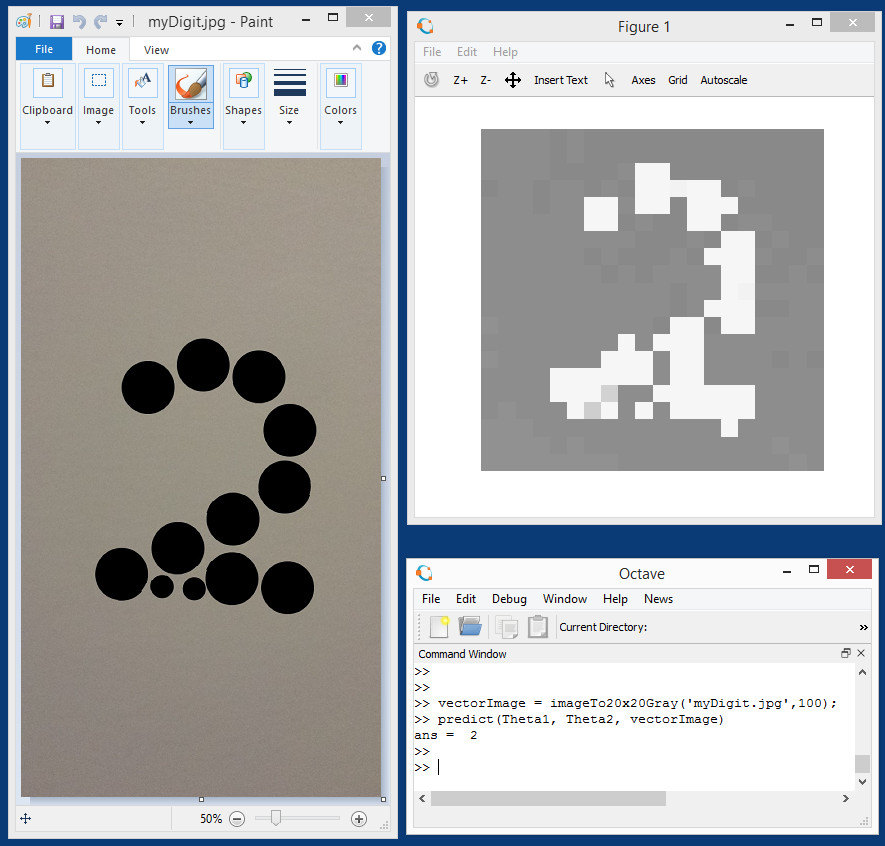
\includegraphics[width=\textwidth]{W5_a}
         \caption{Digit 2}
         \label{fig:W5_a}
     \end{subfigure}
     \hfill
     \begin{subfigure}[b]{0.47\textwidth}
         \centering
         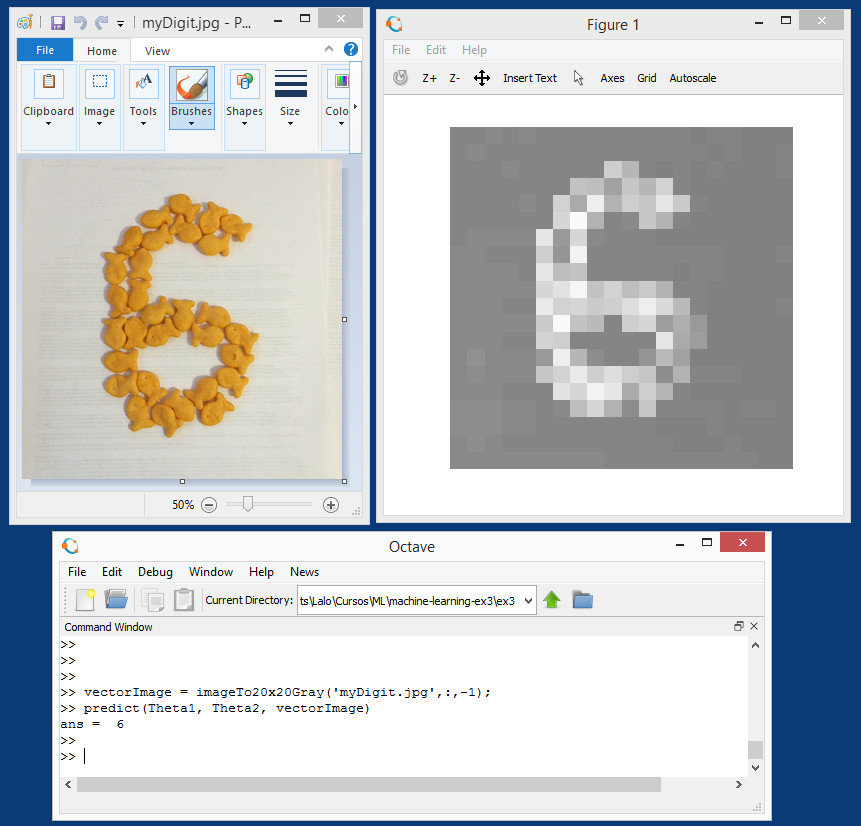
\includegraphics[width=\textwidth]{W5_b}
         \caption{Digit 6}
         \label{fig:W5_b}
     \end{subfigure}
     \hfill
     \begin{subfigure}[b]{0.47\textwidth}
         \centering
         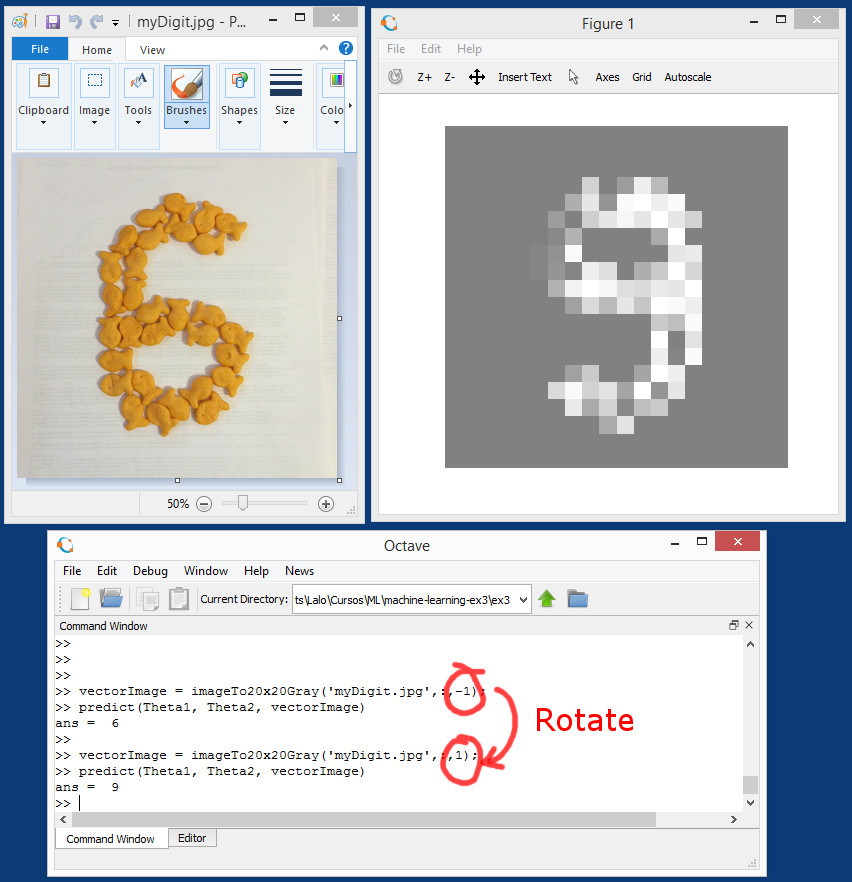
\includegraphics[width=\textwidth]{W5_c}
         \caption{Digit 9}
         \label{fig:W5_c}
     \end{subfigure}
     \hfill
     \begin{subfigure}[b]{0.47\textwidth}
         \centering
         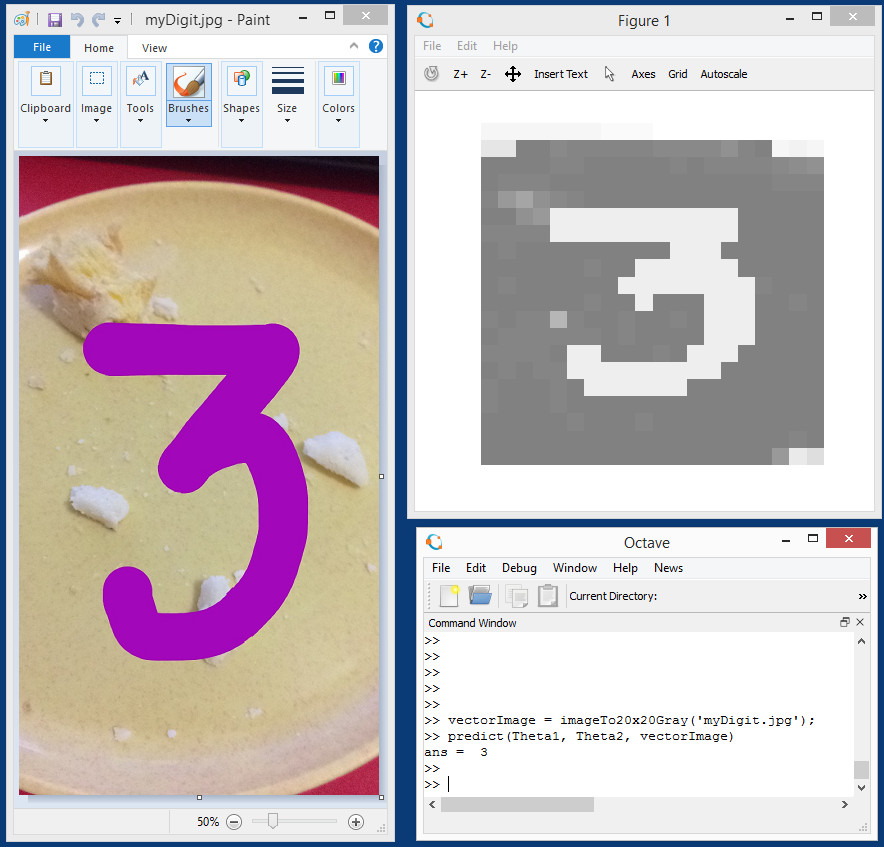
\includegraphics[width=\textwidth]{W5_d}
         \caption{Digit 3}
         \label{fig:W5_d}
     \end{subfigure}
        \caption{Photo Gallery}
        \label{fig:W5_gallery}
\end{figure}
Digit 6 inverted is digit 9 (figure \ref{fig:W5_c}). This is the same photo of a six but rotated. Also, changed the contrast multiplier from 5 to 20. You can note that the gray background is smoother.
